% ============================================================
% Conteúdo acadêmico puro do documento "Modelo de Banco de Dados".
% SEM \documentclass, \begin{document}/\end{document} nem título —
% pensado para ser reaproveitado via \input{} tanto no documento
% modular quanto, futuramente, no TCC principal.
%
% Fonte do conteúdo: Modelo_Banco_de_Dados.md e schema.sql (nesta
% mesma pasta), que descrevem o estado atual da persistência
% (SQLite) — já migrada a partir do antigo modelo CSV/JSON.
% ============================================================

\section{Apresentação do Modelo de Dados}

O RadarTorres é um protótipo que detecta alvos por sensoriamento, seleciona automaticamente a
torre mais adequada e permite o acionamento manual ou automático de um indicador demonstrativo.
Para cumprir esse papel, o sistema precisa preservar, entre execuções, dados de naturezas
distintas: contas de usuário e seus perfis de acesso, o histórico de objetos detectados pelo
radar, a auditoria de toda ação de acionamento e de toda troca de modo de operação, e as
preferências de interface de cada usuário.

Por não depender de um servidor de banco de dados, o protótipo prioriza simplicidade de
instalação e execução local/offline — coerente com o estágio atual do projeto (protótipo
acadêmico, uso demonstrativo). As seções seguintes descrevem a tecnologia de persistência
empregada, por que essa escolha foi feita, as especificações técnicas do SGBD e as entidades
e relacionamentos do modelo atual.

\section{Tecnologia e Implementação}

O protótipo utiliza \textbf{SQLite} como único mecanismo de persistência. O contêiner de injeção
de dependência (\texttt{App.xaml.cs:141--146}) registra uma implementação \texttt{Sqlite*Repository}
para cada uma das 5 tabelas do sistema (\texttt{Usuario}, \texttt{ObjetoDetectado},
\texttt{AcaoRealizada}, \texttt{ModoAtualTorre}, \texttt{PreferenciasUsuario}). Não existem mais
classes de persistência em CSV no repositório — a migração CSV~$\rightarrow$~SQLite, antes
descrita como plano futuro, já foi concluída.

O arquivo de dados reside em \texttt{\%AppData\%}\allowbreak\texttt{\textbackslash
RadarTorres}\allowbreak\texttt{\textbackslash Data\textbackslash radartorres.db} (pasta do
usuário do Windows, sem exigir privilégio de administrador). Falhas de escrita são enfileiradas
em \texttt{pending-writes.sql} (\texttt{PendingWriteQueue.cs}) e reaplicadas automaticamente na
próxima inicialização, evitando perda silenciosa de dados.

\subsection{Especificações técnicas do SGBD}

\begin{table}[htbp]
  \centering
  \caption{Especificações técnicas da persistência}
  \label{tab:specs}
  \small
  \renewcommand{\arraystretch}{1.25}
  \begin{tabular}{p{3.8cm}p{9.4cm}}
    \hline
    \textbf{Item} & \textbf{Valor} \\
    \hline
    SGBD & SQLite (embarcado, arquivo único, sem servidor) \\
    Driver/linguagem de acesso & \texttt{Microsoft.Data.Sqlite} versão \textbf{9.0.0}, consumido em
    C\#/.NET~9 \\
    Versão do engine & Embutida no pacote via \texttt{SQLitePCLRaw}; não pinada separadamente pelo
    projeto \\
    Codificação & UTF-8 (padrão SQLite para colunas \texttt{TEXT}) \\
    Collation & \texttt{BINARY} (padrão; nenhuma coluna usa \texttt{COLLATE} customizado) \\
    Integridade referencial & \texttt{PRAGMA foreign\_keys = ON} \\
    Modelo de concorrência & Single-writer / multi-reader (padrão SQLite, arquivo local) \\
    \hline
  \end{tabular}
\end{table}

\subsection{Por que SQLite: argumento de segurança e leveza}
\label{sec:justificativa}

A escolha do SQLite para o RadarTorres não é um atalho de conveniência — decorre diretamente do
perfil de execução do sistema: um aplicativo desktop único, instalado na máquina do operador,
sem rede corporativa, sem múltiplos servidores concorrentes e com volume de dados compatível com
um protótipo demonstrativo. Dentro desse perfil, SQLite oferece a combinação de
\textbf{segurança} e \textbf{leveza} que um SGBD cliente-servidor (PostgreSQL, SQL Server, MySQL)
não justificaria:

\begin{itemize}
  \item \textbf{Superfície de ataque menor:} por não expor porta de rede nem processo de servidor
  separado, o SQLite elimina uma classe inteira de riscos (varredura de porta, autenticação de
  rede, man-in-the-middle entre aplicação e banco) — o banco só é acessível por quem já tem acesso
  ao arquivo local, no próprio disco do usuário.
  \item \textbf{Integridade garantida mesmo sendo leve:} \texttt{PRAGMA foreign\_keys = ON} aplica
  chaves estrangeiras reais, e o mecanismo ACID nativo do SQLite (transações atômicas por arquivo)
  evita corrupção parcial em caso de queda de energia ou encerramento abrupto — sem exigir o
  processo e a configuração de um SGBD completo para obter essa garantia.
  \item \textbf{Senhas nunca em texto puro:} a camada de aplicação usa PBKDF2-HMACSHA256
  (100.000 iterações, salt de 128 bits por usuário), independente do SGBD escolhido — mas a
  ausência de um servidor de rede reduz também a superfície onde esse hash poderia ser
  interceptado em trânsito.
  \item \textbf{Zero instalação, zero administração:} não há usuário de banco, senha de
  administrador de SGBD, porta a abrir no firewall ou serviço do Windows a manter — o único
  artefato é um arquivo \texttt{.db} na pasta do próprio usuário, reduzindo pontos de falha e de
  configuração incorreta (más práticas de hardening de servidor não se aplicam a um banco que não
  existe como servidor).
  \item \textbf{Leveza compatível com o hardware do protótipo:} o motor SQLite é embutido no
  processo da aplicação (\texttt{Microsoft.Data.Sqlite}), sem overhead de IPC/rede e sem consumo
  de memória de um processo de SGBD separado — adequado ao uso em uma estação de operação única,
  sem exigir infraestrutura dedicada de banco de dados.
  \item \textbf{Resiliência a falhas sem complexidade adicional:} a fila de escritas pendentes
  (\texttt{PendingWriteQueue.cs}) cobre o único cenário de falha relevante para um arquivo local
  (banco temporariamente indisponível/bloqueado), sem precisar de um cluster ou réplica para
  alta disponibilidade — desnecessário na topologia de nó único do RadarTorres.
\end{itemize}

Em resumo: para o escopo atual do RadarTorres — uma aplicação local, de usuário único por
instalação, sem exposição a rede — o SQLite entrega as garantias de integridade e auditoria que
o sistema exige, com a menor superfície de ataque e o menor custo operacional possíveis. Caso o
projeto evolua para múltiplos usuários concorrentes em rede, essa decisão seria revisitada em
favor de um SGBD cliente-servidor.

\section{Principais Entidades do Sistema}

\begin{table}[htbp]
  \centering
  \caption{Tabelas do schema atual (SQLite)}
  \label{tab:entidades}
  \small
  \renewcommand{\arraystretch}{1.2}
  \begin{tabular}{p{3.6cm}p{8.4cm}}
    \hline
    \textbf{Tabela} & \textbf{Finalidade} \\
    \hline
    usuarios & Contas de acesso, perfil (Administrador/Operador/Visualizador) e autenticação \\
    objetos\_detectados & Histórico de ocorrências de detecção (radar e câmera, por quadrante) \\
    ocorrencia\_estados & Auditoria das transições de estado de cada ocorrência (só inserção) \\
    cameras & Câmera responsável por cada quadrante (Q1--Q4) \\
    acoes\_realizadas & Auditoria de acionamentos efetivamente executados (só inserção) \\
    modo\_atual\_torre & Auditoria de troca de modo de operação (só inserção) \\
    preferencias\_usuario & Preferências de interface por usuário (tema, idioma, sidebar) \\
    \hline
  \end{tabular}
\end{table}

\section{Modelo e Relacionamentos}
\label{sec:modelo}

A Figura~\ref{fig:der} reproduz o Diagrama Entidade-Relacionamento do schema atual (arquivo
\texttt{Modelo\_Banco\_de\_Dados.md} e \texttt{schema.sql}, nesta mesma pasta).

\texttt{usuarios} se relaciona 1:1 com \texttt{preferencias\_usuario} (chave \texttt{UsuarioId},
igual a \texttt{usuarios.Id}) e 1:N com \texttt{modo\_atual\_torre} — agora por chave estrangeira
real (\texttt{ID\_USER} $\rightarrow$ \texttt{usuarios.Id}), com \texttt{PRAGMA foreign\_keys =
ON} garantindo a integridade. \texttt{objetos\_detectados} se relaciona 1:N com
\texttt{acoes\_realizadas} (quando há alvo associado ao acionamento) e com
\texttt{ocorrencia\_estados} (histórico de transição); \texttt{cameras} se relaciona 1:N com
\texttt{objetos\_detectados} pelo quadrante monitorado. \texttt{objetos\_detectados} não possui
relacionamento persistido com \texttt{usuarios} — o campo \texttt{Dispositivo} identifica a fonte
da detecção (ex.: ``Arduino'', ``Simulador''), não um usuário.

\begin{figure}[htbp]
  \centering
  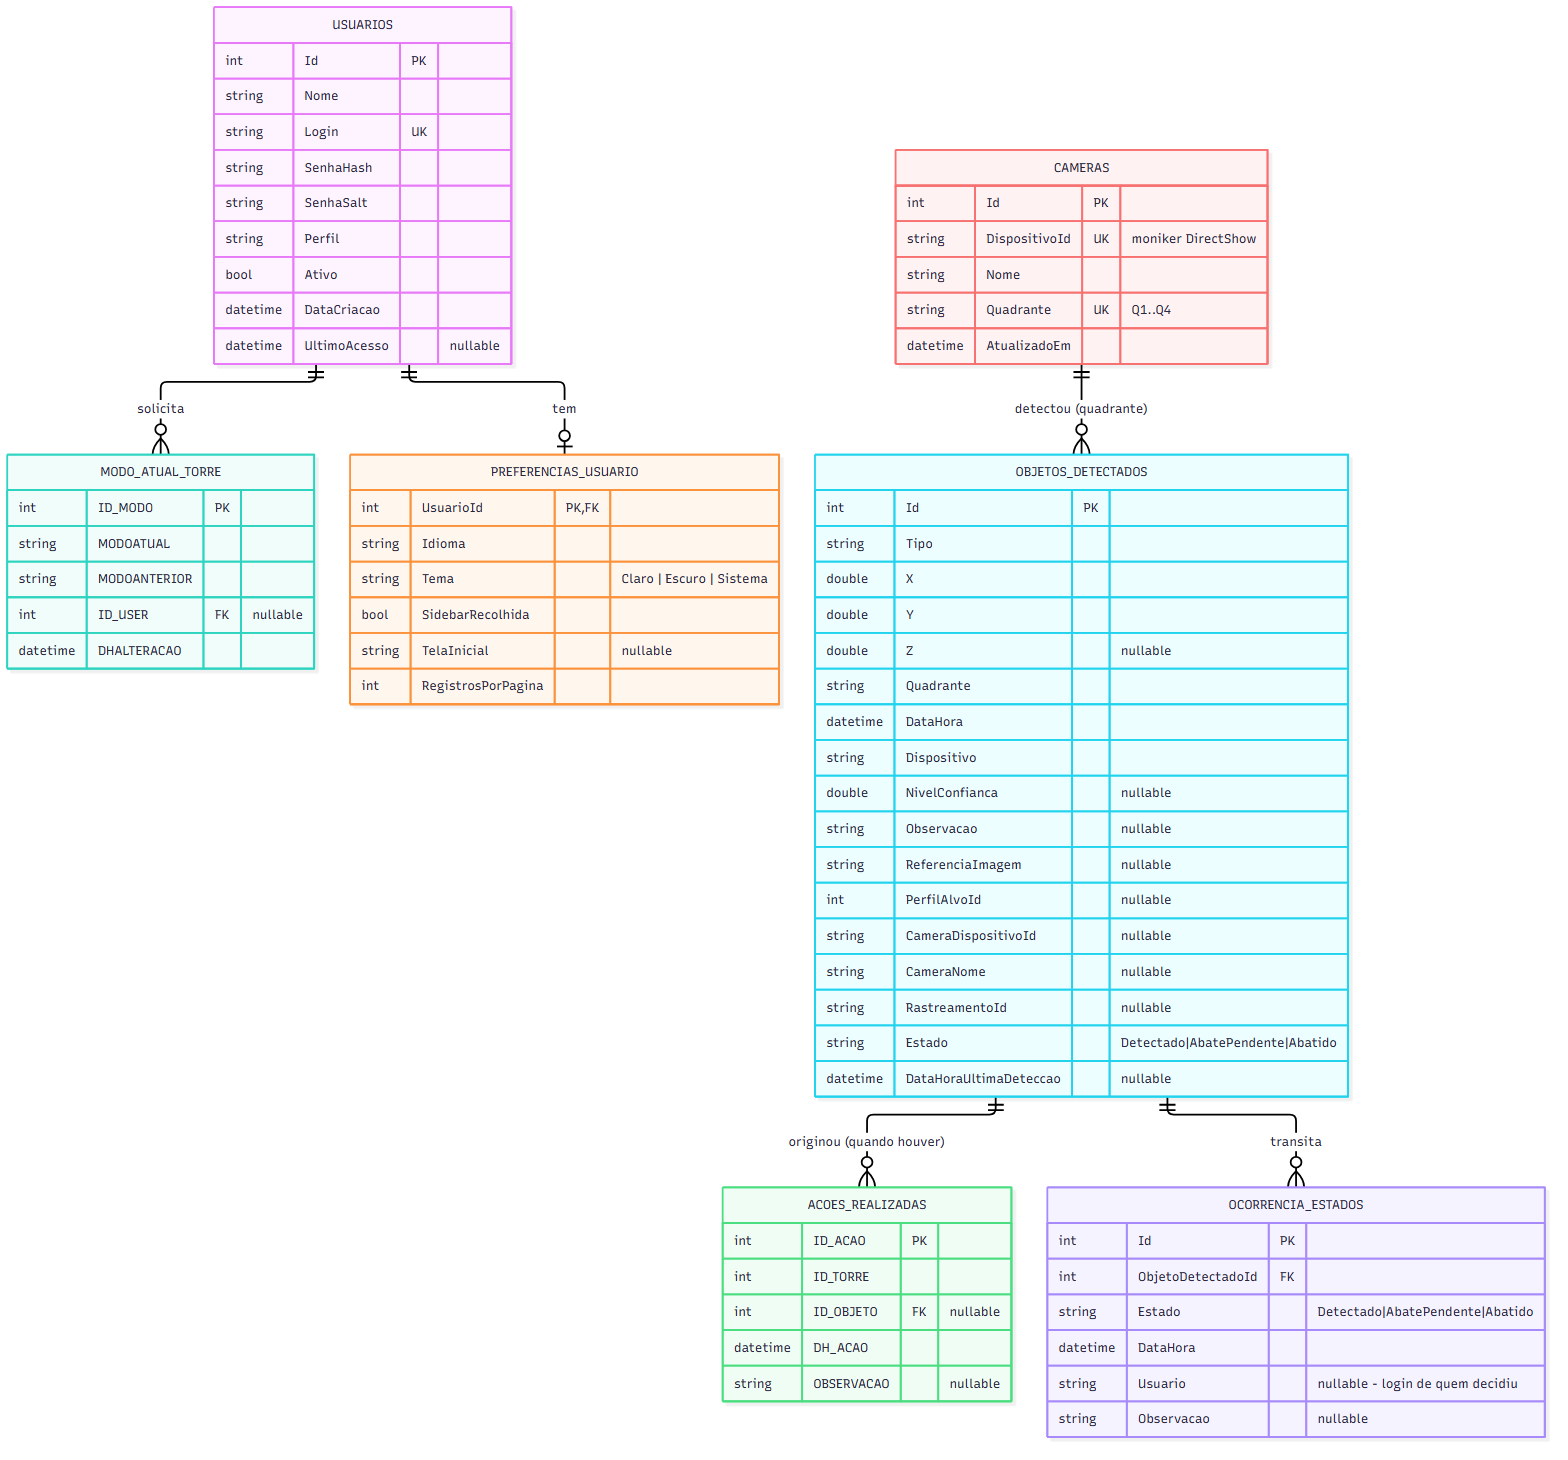
\includegraphics[width=\textwidth]{DER_SQLite.png}
  \caption{Modelo de dados atual (SQLite) — diagrama entidade-relacionamento levantado a partir
  do schema em produção (\texttt{schema.sql}).}
  \label{fig:der}
\end{figure}

\section{Índices}

Além das chaves primárias e das restrições \texttt{UNIQUE} (\texttt{usuarios.Login},
\texttt{preferencias\_usuario.UsuarioId}), o schema define os índices da Tabela~\ref{tab:indices}
para as consultas mais frequentes da aplicação (ordenação por data/hora, filtragem por torre e
por usuário).

\begin{table}[htbp]
  \centering
  \caption{Índices definidos em \texttt{schema.sql}}
  \label{tab:indices}
  \small
  \renewcommand{\arraystretch}{1.2}
  \begin{tabular}{p{5.2cm}p{4.2cm}p{2.4cm}}
    \hline
    \textbf{Índice} & \textbf{Tabela / coluna(s)} & \textbf{Tipo} \\
    \hline
    idx\_acoes\_realizadas\_torre & acoes\_realizadas (ID\_TORRE) & normal \\
    idx\_objetos\_detectados\_datahora & objetos\_detectados (DataHora) & normal \\
    idx\_acoes\_realizadas\_datahora & acoes\_realizadas (DH\_ACAO) & normal \\
    idx\_modo\_atual\_torre\_usuario & modo\_atual\_torre (ID\_USER) & normal \\
    idx\_objetos\_detectados\_perfil & objetos\_detectados (PerfilAlvoId) & normal \\
    idx\_ocorrencia\_estados\_objeto & ocorrencia\_estados (ObjetoDetectadoId) & normal \\
    idx\_objetos\_detectados\_rastreamento & objetos\_detectados (RastreamentoId, Quadrante) &
    único, parcial \\
    idx\_cameras\_dispositivo & cameras (DispositivoId) & único \\
    idx\_cameras\_quadrante & cameras (Quadrante) & único \\
    \hline
  \end{tabular}
\end{table}

O índice único parcial \texttt{idx\_objetos\_detectados\_rastreamento} (\texttt{WHERE
RastreamentoId IS NOT NULL}) é o que impede duplicar a ocorrência do mesmo acompanhamento num
mesmo quadrante, inclusive quando várias câmeras processam em paralelo — sem restringir o radar,
que não gera \texttt{RastreamentoId} e pode repetir quadrante legitimamente.

\section{Conclusão}

A persistência atual, baseada em SQLite, atende ao estágio de protótipo do RadarTorres com
integridade referencial real, auditoria consistente e instalação/execução totalmente locais. A
escolha do SGBD — detalhada na Seção~\ref{sec:justificativa} — equilibra segurança (menor
superfície de ataque, ausência de servidor exposto) e leveza (sem instalação ou administração de
infraestrutura de banco), dentro do perfil de uso de nó único do sistema. O uso de uma interface
de repositório dedicada para cada entidade mantém a camada de dados desacoplada das demais
camadas da aplicação, viabilizando uma eventual migração futura para um SGBD cliente-servidor
sem exigir mudanças em ViewModels ou Services.

\section*{REFERÊNCIAS}
\small
\raggedright
[REFERÊNCIA BIBLIOGRÁFICA A INSERIR]
